\documentclass[10pt]{article}

\usepackage{lipsum}
\usepackage{url}
\usepackage{float}
\usepackage{amsmath}
\usepackage{enumitem}
\usepackage{graphicx}
\usepackage{caption}
\usepackage{subcaption}
\usepackage{rotating}
\usepackage{geometry}
\usepackage{listings}
\usepackage{hyperref}
\usepackage[T1]{fontenc}
\usepackage[numbered]{matlab-prettifier}

\newcommand{\documentTitle}{Lab 3 --INSERT TITLE}
\newcommand{\documentAuthor}{Andrew Pham, Aneel Damaraju}
\newcommand{\courseTitle}{ELEC 240}
\newcommand{\testDate}{September 19,2018}
\newcommand{\reportDate}{September 26, 2018}

\geometry{margin=1in}
\lstset{
    tabsize=4,
    basicstyle={\ttfamily},
    captionpos=b,
    belowskip=1em,
    aboveskip=1em,
    numbers=left,
	escapechar=\@,
}

\title{
    \textbf{\courseTitle} \\
    \textbf{\documentTitle} \\
    \bigskip
    \textbf{\large{Test performed: \testDate}} \\
    \textbf{\large{Report submitted: \reportDate}} \\
    \bigskip
    \bigskip
}
\author{\documentAuthor}
\date{}

\begin{document}

\maketitle

\newpage

\section{Objective}

In the first section of this lab, we explored running various amounts of AC and DC current through a voltage divider of different voltages. We also used a potentiometer as a voltage divider and verified its accuracy. In the second portion of this lab, we measured the transfer function of an RC Circuit by measuring its phase and amplitude with various input frequencies, and we then compared it with the calculated transfer function generated using MATLAB. Finally, we simulated two different RC circuits using LTSpice software and plotted the gain of the circuit at various input frequencies. 

%\textit{Note (To be deleted): Think of this test report as a document with your peers as your readers. This means you can assume a similar knowledge background as you. Your readers should be able to easily understand what is going on, and also be able to repeat your lab results based on your document and all references you cite.}

%\textit{For the Objective section, identify the test you performed and its objectives. The objectives of the test are important to state because they are usually analyzed in the conclusion to determine whether the test succeeded.}

\section{Materials}

\begin{itemize}
	\item Virtual Bench (Software, Oscilloscope, Function Generator, DC Power Supply)
	\item Computer with LTSpice Software 
	\item BNC Male to Clips cord
	\item BNC T connector
	\item Oscilloscope Probe
	\item Breadboard
	\item 2 10 cm length wires (with 6 mm stripped on each end)
	\item Digital Multimeter
	\item 10$k\Omega$ potentiometer
	\item 2 47$\Omega$ resistors
	\item 2 1$M\Omega$ resistors
	\item 2.2 $k\Omega$ resistor
	\item 2.2$\mu F$ resistor
	
\end{itemize}

\medskip

%\textit{Note (To be deleted): Provide a bullet point list of components, software tools, and hardware (such as the NI VirtualBench or DMM) used during the lab}

\section{Test Description}
In Part A of Experiment 3.1, we explored the freuqency range that the DMM on the Virtual Bench could usefully measure by outputting a sine wave from the function generator and recording the maximum voltage recorded by the DMM hooked up to this outputted sine wave. In Part B, we measured the output of a voltage divider and observed how circuits in reality deviate from ideal circuits. In Part C, we used a poteniometer as a voltage divider and verified that turning the slider in equal increments would proportionally increase the resistance of the potentiometer. 

In Part A of Experiment 3.2, we measured the transfer function of an RC Circuit that we wired on the breadboard by inputting various AC frequencies and measuring and plotting the resulting voltage signal. In Part B, we simulated an RC circuit by creating a virtual circuit on LTSpice. We then performed AC analysis by plotting the gain of the RC Circuit over a wide frequency range.  


\medskip

%\textit{Note (To be deleted): This section provides a summary of the test your team performed. Give enough information so readers can understand what you did, but do not go into the details of every step.}

\subsection{Pre-Lab Calculations and Schematics}

No pre-lab calculations were needed, but an understanding of how to measure a transfer function of an AC circuit was needed. Depicted below in Fig. \ref{measurement} is the desired oscilloscope output overlay needed to measure the transfer function:
\begin{centering}
	\begin{figure} [H]
		\centering
		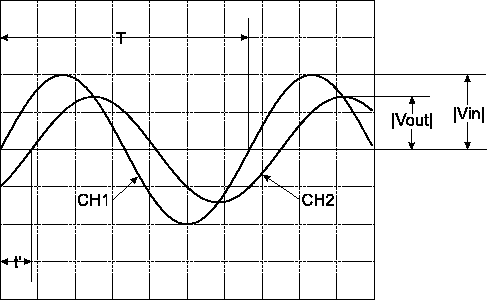
\includegraphics[scale=0.5]{images/measurementexample.png}
		\caption{Circuit Output Signal Overlayed with Function Generator Output}
		\label{measurement}
	\end{figure}
\end{centering}

To measure the transfer function at a given frequency, we needed to measure both $|V_{IN}|$ and $|V_{OUT}|$, which was achieved by measuring the height of the peaks of CH1 and CH2. To measure the phase $\Phi$, we measured the horizontal distance between the peaks of CH1 and CH2. With this technique, we are able to perform AC circuit analysis in Part A of Experiment 3.2. 
\medskip

%\textit{Note (To be deleted): Include the homework pre-calculations and schematics that serve as the initial setup for the test. Briefly explain the importance of each item you include. You may want to number your equations/figures so you can refer to them in later sections. Including photos of handwritten work is okay.}

\section{Results and Discussion}

Your text here

\medskip

\textit{Note (To be deleted): The heart of your report is the presentation of your results and a discussion of those results. In your discussion, you should not only analyze your results, but also discuss the implications of those results.}

\section{References}

Your text here

\medskip

\textit{Note (To be deleted): List any datasheets, websites, lab procedure, etc. used during the lab.}

\section{Conclusion}

Your text here

\medskip

\textit{Note (To be deleted): While the ``Results and Discussion'' section focused on the test results individually, the ``Conclusion'' discusses the results in the context of the entire experiment. Usually, the objectives given in the ``Introduction'' are reviewed to determine whether the experiment succeeded. If the objectives were not met, you should analyze why the results were not as predicted.}

\section{Errors}

Your text here

\medskip

\textit{Note (To be deleted): Briefly list sources of error and discuss how to eliminate or deal with them}

\end{document}
